%
% File acl2024.tex
%
%% Based on the style files for ACL 2023, which were
%% Based on the style files for ACL 2022, which were
%% Based on the style files for ACL 2021, which were
%% Based on the style files for ACL 2020, which were
%% Based on the style files for ACL 2019, which were based on ACL 2018, NAACL 2018, ACL 2017, ACL 2016, ACL 2015, ACL 2014, ACL 2013
%% Based on the style files for EACL 2009 and We use the official ACL class
%
% Iteration 2: duplicated from report.tex (the compiled main paper) and extended
% with the Bangladesh (BD) cross-jurisdictional external-validation study. The
% original report.tex / main.tex / compiled PDF are untouched by this file.

\documentclass[11pt]{article}
\usepackage[T1]{fontenc}
\usepackage[utf8]{inputenc}
\usepackage{acl}
\usepackage{times}
\usepackage{latexsym}
\usepackage{graphicx}
\usepackage{booktabs}
\usepackage{multirow}
\usepackage{array}
\usepackage{tabularx}

\newcommand\BibTeX{B\textsc{ib}\TeX}

\title{Leakage-Aware Privacy-Practice Classification: A Comparative Study of Classical and Neural Models under Policy-Disjoint Evaluation }

\author{%
\begin{tabular}{cc}
Nafiz Ahmed Nafi & Priom Halder \\
{\small\normalfont\texttt{nafiz.ahmed.nafi@g.bracu.ac.bd}} &
{\small\normalfont\texttt{priom.halder@g.bracu.ac.bd}} \\[0.6em]
MD. Amirul Islam Sadat & Samiha Tasnim Orthi \\
{\small\normalfont\texttt{amirul.islam.sadat@g.bracu.ac.bd}} &
{\small\normalfont\texttt{samiha.tasnim.orthi@g.bracu.ac.bd}} \\[0.8em]
\multicolumn{2}{c}{\normalfont Department of Computer Science and Engineering, BRAC University}
\end{tabular}%
}

\begin{document}

\maketitle

\begin{abstract}
Privacy policies govern how personal data is collected, shared, and retained, yet most users never read them in full. We study automatic classification of annotated privacy-policy spans into eight data-practice categories using the OPP-115 corpus (17,343 labeled spans, 115 policies). TF-IDF is used for completed classical experiments; a Word2Vec pipeline was implemented but not executed for completed downstream classification. Models span three classical approaches (Random Forest, Logistic Regression, Naive Bayes) and seven neural architectures (SimpleRNN, GRU, LSTM, their bidirectional variants, and partially fine-tuned BERT Base). Our central contribution is systematic comparison of two evaluation protocols: conventional row-level stratified split and policy-disjoint split that holds entire policies out of training. Because privacy policies reuse boilerplate language, the row-level split inflates macro-F1 by 0.015--0.123 depending on model and changes apparent ranking. Under honest policy-disjoint evaluation, BERT Base achieves highest macro-F1 (0.706), narrowly ahead of Naive Bayes (0.701), showing smallest evaluation-protocol gap. We checkpoint the policy-disjoint BERT Base classifier for the first time and apply it, without retraining, to real privacy policies from 35 Bangladeshi companies never seen during training. Of 3,120 classified sentences from 26 companies with usable extracted text, the predicted category distribution largely preserves OPP-115's shape (First Party Collection/Use dominant in both), with two notable divergences: Data Security is over-predicted by 6.9 percentage points at above-average confidence (0.740), plausibly a real sectoral effect, while User Choice/Control is under-predicted by 4.8 points at the lowest confidence of any category (0.550), a pattern consistent with domain shift rather than a confirmed disclosure gap. Results suggest document-grouped evaluation should be standard for text classification tasks built on corpora with reused or template-based language, and that a trained classifier's per-category confidence is a usable, label-free signal for diagnosing domain shift when applying it outside its training distribution.
\end{abstract}

\section{Introduction}

Privacy policies are the main legal instrument through which organizations disclose how they collect, use, share, and retain personal data. In practice, they are long, formulaically written, inconsistently structured, and surveys of user behavior repeatedly find that almost nobody reads one in full before consenting~\cite{mcdonald-cranor-2008-cost}. Automatically mapping policy text onto a standardized taxonomy of data practices would enable downstream tools to summarize policies at a glance, flag GDPR or CCPA-relevant language, or allow researchers to compare practices at corpus scale. This is a multi-class text classification problem and not a saturated task: privacy language is technical, class frequencies are heavily skewed, and single clauses often express more than one practice simultaneously.

We build our study on the OPP-115 corpus~\cite{wilson-etal-2016-creation}, containing 115 real-world website privacy policies annotated by legal experts against a fixed schema of data-practice categories. We treat each annotated span as one classification instance labeled with one of eight practice categories.

A less obvious property of this corpus motivates the paper's central contribution. Privacy policies reuse legally vetted boilerplate language across unrelated organizations---template clauses drafted by the same law firm recur verbatim across dozens of policies. A conventional row-level train/test split ignores this structure and can place near-identical boilerplate on both sides, letting a model score well by recognizing memorized phrases rather than by learning what privacy language of a given category actually looks like. This is an instance of the broader evaluation-leakage problem documented in NLP~\cite{gorman-bedrick-2019-need, lewis-etal-2021-question}.

Iteration 1 of this work (summarized in Sections~\ref{sec:methodology}--\ref{sec:conclusion} below) answered a question internal to OPP-115: which representation and architecture classify a policy span best, and how much does the evaluation protocol itself change the answer. This iteration asks a question external to OPP-115: \textbf{does a classifier trained entirely on US company policies transfer to privacy policies from a market OPP-115 never sampled?} Section~\ref{sec:bd} reports that study.

\subsection{Research Questions}

\begin{itemize}
\item \textbf{RQ1:} How does a conventional row-level split change measured performance relative to a policy-disjoint split for the same model?
\item \textbf{RQ2:} How does this evaluation-protocol gap vary across classical, recurrent, and transformer architectures?
\item \textbf{RQ3:} Which model achieves the best macro-F1 on entirely unseen policies?
\item \textbf{RQ4 (Applied on Bangladeshi Company Privacy Policy):} Does the best policy-disjoint model's predicted category distribution, applied to real Bangladeshi company privacy policies, plausibly track OPP-115's disclosure patterns, and can per-category prediction confidence distinguish a likely domain-shift artifact from a likely real difference?
\end{itemize}

\subsection{Contributions}

\begin{enumerate}
\item A leakage-aware evaluation framework contrasting row-level and policy-disjoint splits across ten models spanning four architecture families.
\item An empirical finding that the evaluation-protocol gap varies substantially across model families.
\item Full implementation of the required classical and neural suite, with implementation gaps documented openly rather than omitted.
\item \textbf{2nd Phase(Application in Bangladeshi Company Policy's dataset)} A checkpointed, reusable artifact of the winning policy-disjoint classifier, and a descriptive cross-jurisdictional transfer study applying it to 35 Bangladeshi companies' privacy policies, using per-category confidence as a label-free diagnostic for domain shift.
\end{enumerate}

Context-aware modeling and imbalance-aware training are left for future work; manually-validated (Tier 2) cross-jurisdictional evaluation is scoped as the immediate next step following this iteration (Section~\ref{sec:future}).

\section{Related Work}

\subsection{Privacy-Policy NLP}

The OPP-115 corpus~\cite{wilson-etal-2016-creation} is the standard manually annotated benchmark for data-practice classification in privacy policies.\ \citet{harkous-etal-2018-polisis} present Polisis, a deep-learning pipeline that classifies policy segments and supports downstream question answering, establishing that neural models can substantially outperform earlier rule-based approaches. Our work differs in focus: rather than proposing a new architecture, we study how the evaluation protocol specifically—whether the split respects document-level structure—changes which architecture appears to win, and, in this iteration, whether a model selected under that honest protocol generalizes across jurisdictions.

\subsection{Classification Models}

TF-IDF paired with classical classifiers remains a strong, fast baseline~\cite{pedregosa-etal-2011-scikit}. Word embeddings such as Word2Vec~\cite{mikolov-etal-2013-efficient} and GloVe~\cite{pennington-etal-2014-glove} enable generalization across related terms. Recurrent architectures including LSTM~\cite{hochreiter-schmidhuber-1997-lstm}, GRU~\cite{cho-etal-2014-learning}, and their bidirectional variants~\cite{schuster-paliwal-1997-bidirectional} model sequential dependencies that bag-of-words representations discard. BERT~\cite{devlin-etal-2019-bert} adds contextual representations from large external corpora before task-specific fine-tuning.

\subsection{Evaluation Leakage and Class Imbalance}

\citet{gorman-bedrick-2019-need} show that re-splitting standard NLP benchmarks changes both absolute scores and relative rankings.\ \citet{lewis-etal-2021-question} document a related failure in question answering where train/test overlap inflates reported accuracy. Our work applies this principle---splits must respect data grouping structure---to a domain where that structure is unusually explicit.\ \citet{johnson-khoshgoftaar-2019-survey} survey class-imbalance mitigations; we adopt macro-F1 as the primary metric and include class-weighted configurations throughout.

\subsection{Cross-Jurisdictional Transfer}

Most published privacy-policy classification work treats its source corpus as a static, single-jurisdiction snapshot; systematic study of how a trained classifier's predictions shift when applied outside that jurisdiction is comparatively underexplored. Section~\ref{sec:bd} is a descriptive step in that direction: reusing a trained classifier as a measurement instrument for a market the training corpus never sampled, rather than proposing a new architecture for the transfer setting itself.

\section{Methodology}
\label{sec:methodology}

\subsection{Dataset and Exploratory Data Analysis}

\subsubsection{Corpus Description}

We use the OPP-115 corpus~\cite{wilson-etal-2016-creation}: 115 website privacy policies, each annotated by three annotators against a fixed schema, later merged at 0.75 overlap-similarity threshold that reproduces the corpus's own 92/23 policy train/test split. We take the longest populated selected span as the classification input and attach its surrounding clause as optional context. Two of the ten original categories (Other and Do Not Track) are dropped, leaving eight:
\begin{enumerate}
\item First Party Collection/Use
\item Third Party Sharing/Collection
\item User Choice/Control
\item Data Security
\item User Access, Edit and Deletion
\item International and Specific Audiences
\item Policy Change
\item Data Retention
\end{enumerate}

\subsubsection{Scale and Distribution}

The working dataset contains 17,343 labeled spans from 3,204 distinct underlying clauses and 115 policies. Of the 17,343 rows, 4,959 are repeated (span, category) pairs, an early signal of the boilerplate reuse that motivates our evaluation design. Annotated spans are short (mean 137 characters; median 15 words); surrounding clauses are longer (median 89 words).

\subsubsection{Class Distribution and Span Lengths}

Figure~\ref{fig:class_dist} shows the class distribution. First Party Collection/Use and Third Party Sharing/Collection together account for 74.7\% of all rows, while Data Retention accounts for only 1.9\%---a 24.3$\times$ imbalance. This is why accuracy is never reported as a standalone metric; every evaluation centers macro-F1 and reports full per-class breakdowns. Span lengths are mostly short, with a long right tail (maximum 1,873 characters); this motivates the 48-token sequence-length cap used for recurrent models, as shown in Figure~\ref{fig:span_length}.

\begin{figure}[t]
\centering
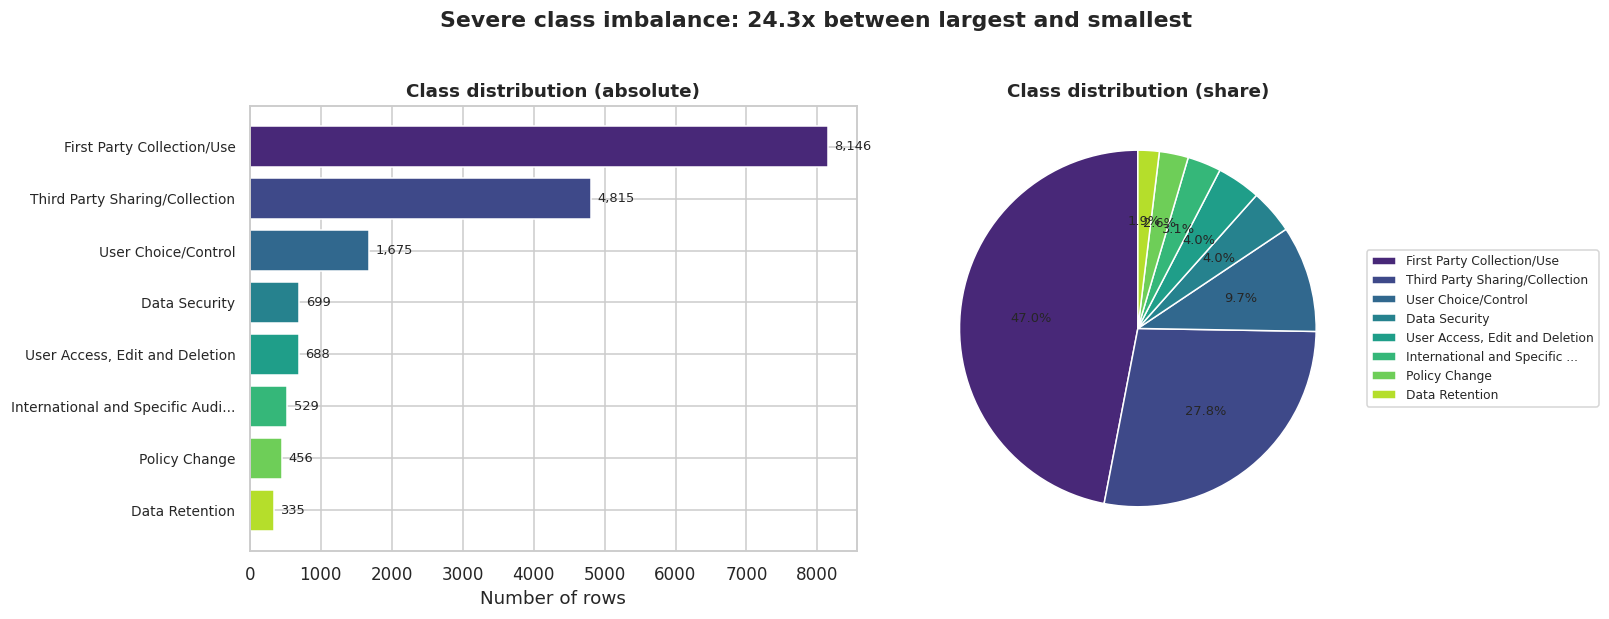
\includegraphics[width=0.95\columnwidth]{figures/class_distribution.png}
\caption{Category distribution over 17,343 spans by (a) absolute count and (b) share of the corpus, highlighting the 24.3$\times$ ratio between the largest and smallest classes.}
\label{fig:class_dist}
\end{figure}

\begin{figure}[t]
\centering
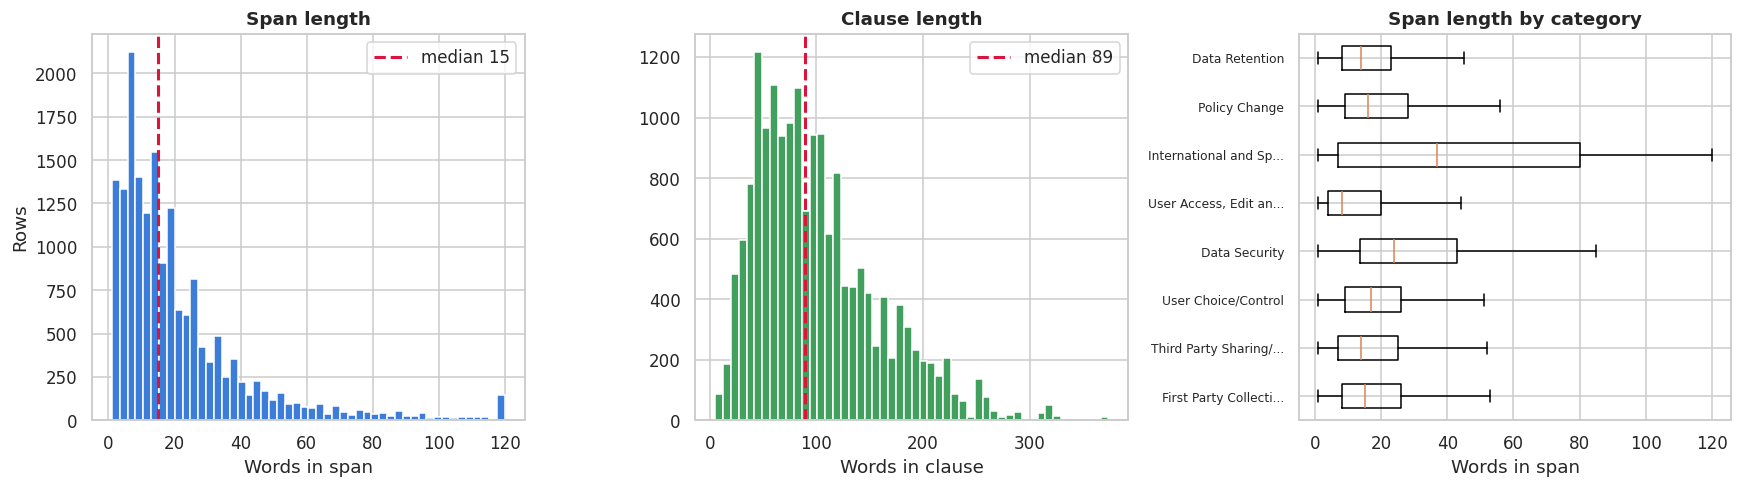
\includegraphics[width=0.95\columnwidth]{figures/span_length.png}
\caption{Span length, clause length, and span length by category, in words. Dashed lines mark the median (15 words for spans, 89 for clauses).}
\label{fig:span_length}
\end{figure}

\subsubsection{Multi-Practice Clauses}

1,119 of 3,204 distinct clauses (34.9\%) carry more than one category simultaneously. For example, a sentence such as ``we collect your email address and may share it with advertising partners unless you opt out'' simultaneously expresses First Party Collection/Use, Third Party Sharing/Collection, and User Choice/Control. This is why the clause is never used as the sole classification input; a clause-level single-label formulation would force one label onto text that legitimately expresses several practices. This same finding is why Section~\ref{sec:bd} segments Bangladeshi policy text at sentence, not clause, granularity before classifying it.

\subsubsection{Boilerplate Reuse}

Under the conventional row-level random split, 113 of 115 policies appear on both sides and 95.2\% of test rows share clause text with some training row. Under the policy-disjoint split, that figure drops to 6.0\%---real-world boilerplate reuse across unrelated organizations rather than an artifact of the split.

This 95.2\% versus 6.0\% difference is the concrete motivation for the dual-scheme evaluation protocol.

\subsection{Preprocessing}

We define five preprocessing variants, each matched to a different downstream representation, as shown in Table~\ref{tab:preprocess}. Every variant first strips HTML markup and replaces URLs and email addresses with placeholder tokens ([URL], [EMAIL]). In the executed pipeline, the base variant was applied to both classical and recurrent models; minimal was applied to BERT Base, and is reused unchanged for Bangladeshi text in Section~\ref{sec:bd} so inference-time preprocessing matches train-time preprocessing exactly.

\begin{table}[t]
\centering
\small
\begin{tabularx}{\columnwidth}{@{}p{1.9cm}XX@{}}
\toprule
\textbf{Variant} & \textbf{Processing} & \textbf{Intended For} \\
\midrule
base & HTML removal, placeholders, lower-case & Classical, RNN (actual) \\
no\_stopwords & base + NLTK stopword removal & Alt. TF-IDF \\
lemmatized & base + WordNet lemmatization & RNN (designed) \\
aggressive & stopwords + lemmatization & Sparse configs \\
minimal & HTML removal, lower-case only & BERT Base \\
\bottomrule
\end{tabularx}
\caption{Preprocessing variants and their intended usage.}
\label{tab:preprocess}
\end{table}

Figure~\ref{fig:preprocess} shows vocabulary size and mean span length for each variant. Stopword removal and lemmatization each reduce vocabulary by roughly one-third relative to base; combining both (aggressive) gives the smallest vocabulary.

\begin{figure}[t]
\centering
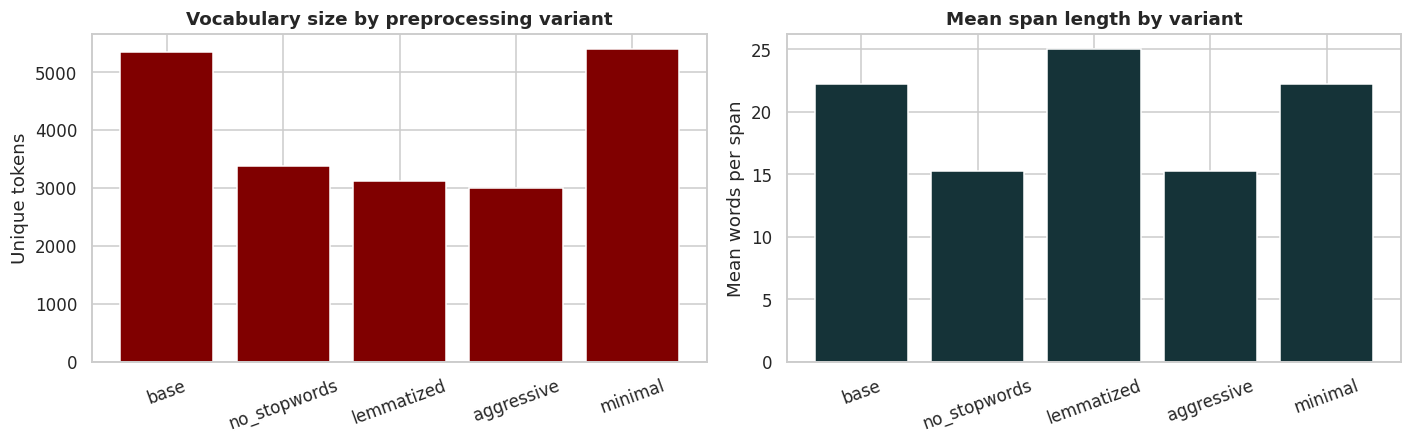
\includegraphics[width=0.95\columnwidth]{figures/preprocessing_variants.png}
\caption{Vocabulary size and mean span length for each preprocessing variant, measured on a 3,000-span sample. Stopword removal and lemmatization each reduce vocabulary by roughly a third relative to base.}
\label{fig:preprocess}
\end{figure}

\subsection{Word Representations}

\subsubsection{TF-IDF (Fully Evaluated)}

We use a 5,000-term vocabulary with unigrams and bigrams, minimum document frequency 5, maximum document frequency 0.8, and sublinear term-frequency scaling~\cite{pedregosa-etal-2011-scikit}. The vectorizer is refit independently on the training portion of each split scheme to prevent vocabulary leakage.

\subsubsection{Word2Vec}

A skip-gram Word2Vec pipeline was implemented using 100-dimensional embeddings, a context window of 5, and minimum token count of 2~\cite{mikolov-etal-2013-efficient}, via Gensim~\cite{rehurek-sojka-2010-software}. However, the Word2Vec pipeline was not executed for completed downstream classification experiment, so no Word2Vec classification results are reported.



\subsection{Model Architectures and Hyperparameter Grids}

Table~\ref{tab:models} summarizes all ten models, their representations, and the configurations tested. For every model and split scheme, model selection uses validation macro-F1 and only the winning configuration is scored on the held-out test set.

\begin{table*}[t]
\centering
\begin{tabular}{@{}llll@{}}
\toprule
\textbf{Model Family} & \textbf{Model} & \textbf{Representation} & \textbf{Configs} \\
\midrule
\multirow{3}{*}{Classical} & Logistic Regression & TF-IDF & 3 \\
 & Random Forest & TF-IDF & 3 \\
 & Naive Bayes & TF-IDF & 3 \\
\midrule
\multirow{6}{*}{Recurrent} & SimpleRNN & Embedding & 3 \\
 & GRU & Embedding & 3 \\
 & LSTM & Embedding & 3 \\
 & Bidirectional SimpleRNN & Embedding & 3 \\
 & Bidirectional GRU & Embedding & 3 \\
 & Bidirectional LSTM & Embedding & 3 \\
\midrule
Transformer & BERT Base & Frozen layers & 3 \\
\bottomrule
\end{tabular}
\caption{Model architectures and hyperparameter configurations (3 configs per model $\times$ 2 schemes = 60 configurations).}
\label{tab:models}
\end{table*}

All six recurrent models share the same design: an embedding layer initialized from scratch, a recurrent or bidirectional recurrent layer, dropout regularization, and a dense softmax head. Input sequences are word-index-encoded from a training-only vocabulary and padded or truncated to 48 tokens. Models are implemented in PyTorch~\cite{paszke-etal-2019-pytorch}; final experiments ran in a CUDA-enabled Python 3.13 environment. BERT Base is fine-tuned via the HuggingFace Transformers library~\cite{wolf-etal-2020-transformers} with token embeddings and first 10 of 12 encoder layers frozen, and input truncated to 64 tokens.

\subsection{Split Schemes}

\subsubsection{Random Split (Leaky Comparison)}

Rows are split 70/15/15 (train/val/test), stratified by category, with no regard for policy origin (12,140/2,601/2,602 rows; 113 of 115 policies appear in both train and test). Reported only as a point of comparison against the honest condition.

\subsubsection{Policy-Disjoint Split (Honest Evaluation)}

Policies, not rows, are the unit of assignment, built from the corpus's own 92/23 policy split (76/16/23 policies; 11,344/2,088/3,911 rows). No policy's rows appear in more than one split. This is the paper's generalization estimate and the scheme used for every model-selection decision, and it is the scheme whose winning model is transferred to Bangladeshi text in Section~\ref{sec:bd}.

\section{Results}

All ten models were trained and evaluated under both split schemes for a combined 60 logged tuning runs (18 classical, 36 recurrent, 6 BERT Base). All numbers are drawn directly from the executed project notebook.

\subsection{Model Comparison}

Table~\ref{tab:results} reports test-set performance under both schemes. Figure~\ref{fig:model_comp} visualizes the comparison.

\begin{table*}[t]
\centering
\small
\setlength{\tabcolsep}{3.5pt}
\begin{tabular}{@{}lccc@{\hspace{1em}}ccc@{}}
\toprule
 & \multicolumn{3}{c}{Random Split (Leaky)} & \multicolumn{3}{c}{Policy-Disjoint (Honest)} \\
\textbf{Model} & Accuracy & Macro-F1 & Weighted-F1 & Accuracy & Macro-F1 & Weighted-F1 \\
\midrule
BERT Base & 0.759 & 0.721 & 0.755 & 0.715 & \textbf{0.706} & 0.714 \\
Naive Bayes & 0.757 & 0.726 & 0.755 & 0.703 & \textbf{0.701} & 0.699 \\
Logistic Regression & 0.774 & 0.753 & 0.771 & 0.679 & 0.692 & 0.677 \\
Random Forest & 0.780 & 0.721 & 0.774 & 0.677 & 0.652 & 0.667 \\
Bidirectional LSTM & 0.760 & 0.684 & 0.757 & 0.670 & 0.608 & 0.666 \\
Bidirectional GRU & 0.764 & 0.700 & 0.761 & 0.633 & 0.586 & 0.634 \\
Bidirectional SimpleRNN & 0.728 & 0.612 & 0.722 & 0.617 & 0.489 & 0.609 \\
GRU & 0.711 & 0.519 & 0.704 & 0.585 & 0.475 & 0.583 \\
LSTM & 0.691 & 0.549 & 0.683 & 0.579 & 0.442 & 0.576 \\
SimpleRNN & 0.482 & 0.172 & 0.408 & 0.386 & 0.131 & 0.336 \\
\bottomrule
\end{tabular}
\caption{Test performance at each model's best validated configuration under both split schemes, ranked by macro-F1 under policy-disjoint evaluation.}
\label{tab:results}
\end{table*}

Under the honest, policy-disjoint scheme, BERT Base reaches the best overall macro-F1 (0.706), narrowly ahead of Naive Bayes (0.701)---a gap of 0.005 that should be read as a near-tie rather than a decisive win. Logistic Regression comes third (0.692). SimpleRNN is the worst model overall (macro-F1 0.131, barely above a majority-class-only baseline), and Random Forest is the weakest of the three classical models (0.652).

Under the leaky random scheme, the picture looks quite different: Logistic Regression appears to lead (0.753) and BERT falls to fourth, behind both Random Forest and Naive Bayes. A concrete instance of the accuracy trap appears within the classical models: Random Forest has the highest accuracy of all ten models under the leaky split (0.780) yet the lowest macro-F1 among the three classical models (0.721)---a pattern consistent with the model benefiting disproportionately from the majority class's repeated boilerplate phrasing.

\begin{figure}[t]
\centering
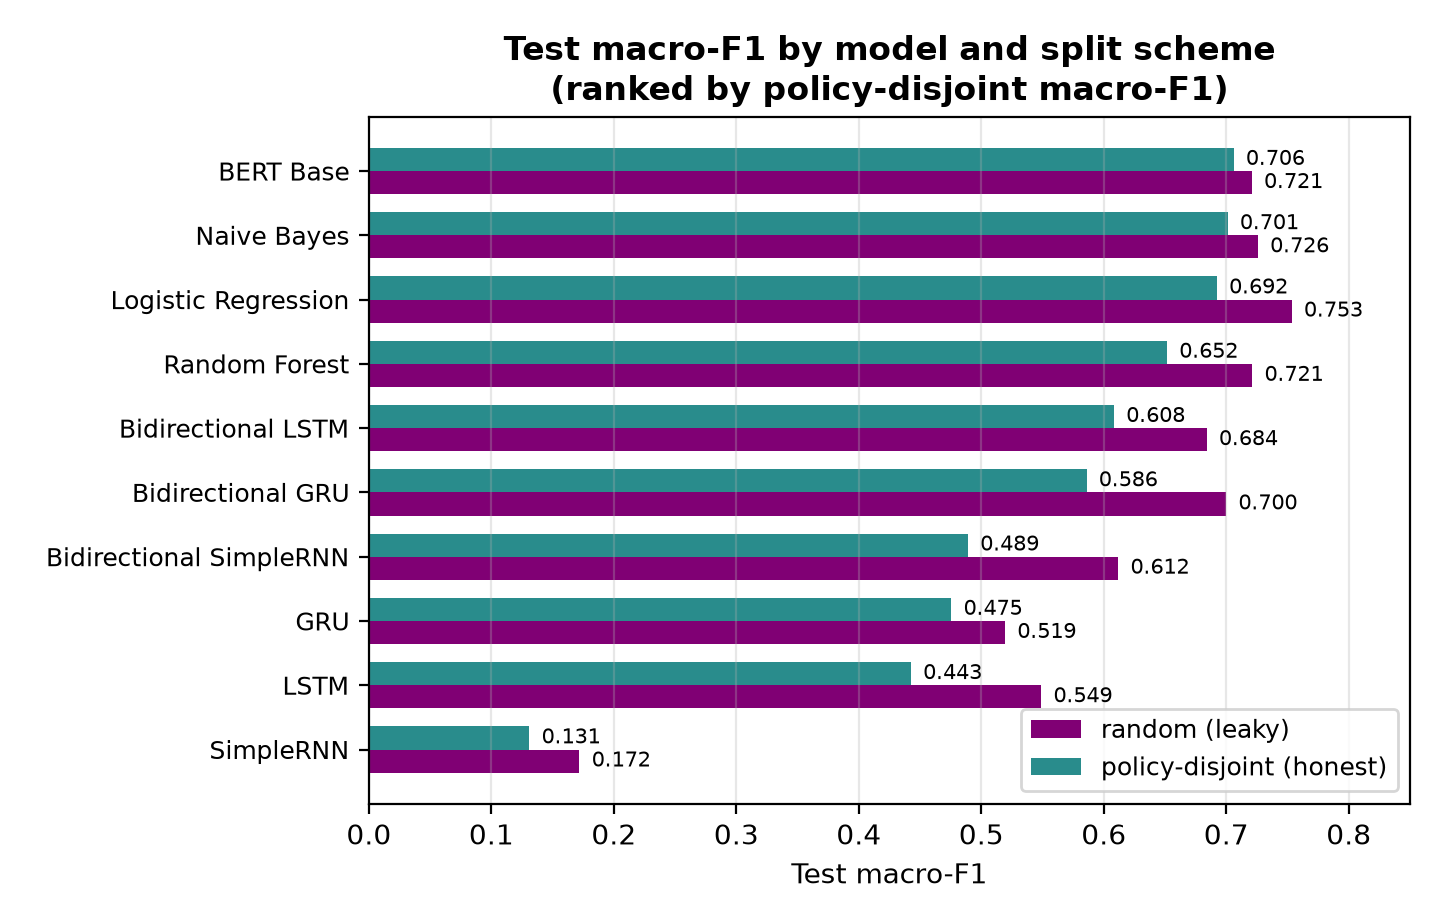
\includegraphics[width=0.95\columnwidth]{figures/model_comparison.png}
\caption{Macro-F1 comparison across all ten models under both split schemes.}
\label{fig:model_comp}
\end{figure}

\subsection{Evaluation-Protocol Gap Analysis}

\begin{figure}[t]
\centering
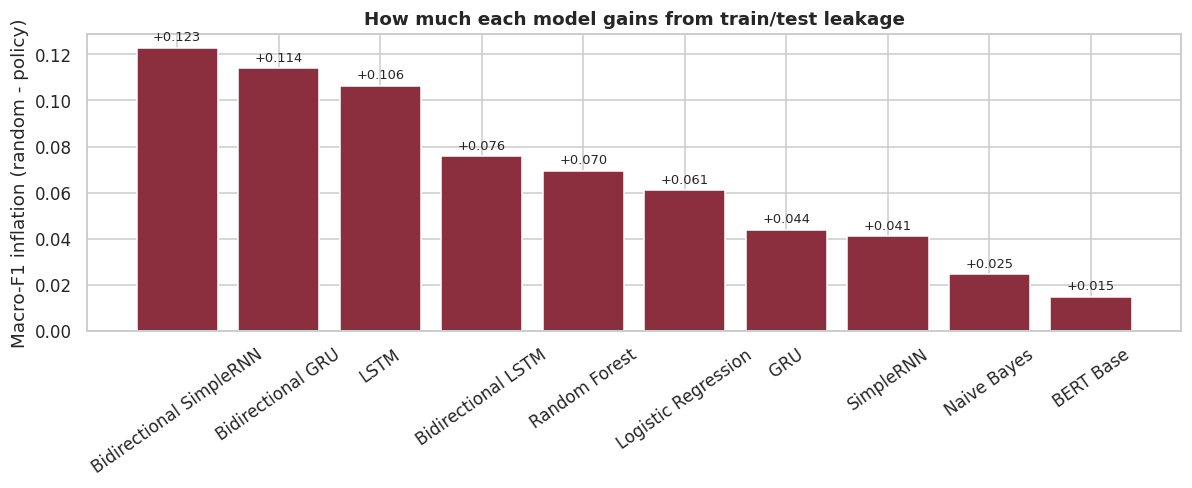
\includegraphics[width=0.95\columnwidth]{figures/leakage_inflation.png}
\caption{Evaluation-protocol macro-F1 gap (random-split score minus policy-disjoint score) by model; larger bars indicate models whose apparent performance depends more heavily on signal not available under honest evaluation.}
\label{fig:gap}
\end{figure}

The macro-F1 gap between the two schemes is shown in Figure~\ref{fig:gap}. We call this an evaluation-protocol gap rather than a pure measure of leakage because the two schemes also differ in test-set size and policy composition; the 95.2\% versus 6.0\% clause-overlap evidence makes leakage the most plausible dominant contributor.

The gap ranges from +0.015 (BERT Base) to +0.123 (Bidirectional SimpleRNN). The three classical models and BERT Base form a comparatively low-gap cluster (+0.015 to +0.070); the six recurrent architectures show both the largest and most variable gap (+0.041 to +0.123), with Bidirectional SimpleRNN, Bidirectional GRU, and unidirectional LSTM each exceeding +0.10.

BERT Base's gap of only +0.015 is consistent with the hypothesis that pretraining on a large external corpus reduces reliance on this dataset's own boilerplate --- the same property that motivates transferring this specific model, rather than a classical baseline, to out-of-distribution Bangladeshi text in Section~\ref{sec:bd}.

\subsection{Per-Class Analysis}

\begin{table}[t]
\centering
\footnotesize
\setlength{\tabcolsep}{3pt}
\begin{tabularx}{\columnwidth}{@{}Xccc@{}}
\toprule
\textbf{Category} & \textbf{Precision} & \textbf{Recall} & \textbf{F1-Score} \\
\midrule
First Party Collection/Use & 0.76 & 0.78 & 0.77 \\
Third Party Sharing/Collection & 0.66 & 0.64 & 0.65 \\
User Choice/Control & 0.56 & 0.62 & 0.59 \\
Data Security & 0.77 & 0.88 & 0.82 \\
User Access, Edit and Deletion & 0.69 & 0.57 & 0.62 \\
International and Specific Audiences & 0.86 & 0.88 & 0.87 \\
Policy Change & 0.91 & 0.77 & 0.84 \\
Data Retention & 0.86 & 0.35 & 0.49 \\
\bottomrule
\end{tabularx}
\caption{Per-class P/R/F1 for BERT Base (policy-disjoint; accuracy 0.715, macro-F1 0.706).}
\label{tab:perclass}
\end{table}

Table~\ref{tab:perclass} reports per-class results for BERT Base under the policy-disjoint test set. The per-class results show no clear relationship between class frequency and classification performance: several relatively small categories achieve high F1 scores, whereas some much larger categories remain more difficult.

Policy Change and International and Specific Audiences are among the smallest categories yet score highest (F1 0.84 and 0.87 respectively), because both use distinctive formulaic vocabulary (``we may update this policy from time to time''; ``residents of the European Economic Area'') that a model learns from relatively few examples.

The dominant error mode is confusion between First Party Collection/Use and Third Party Sharing/Collection: both describe data collection and differ chiefly in who receives the data, a distinction sometimes carried by a single noun phrase within a short span.

Data Retention is the one category where scarcity appears to matter: precision is high (0.86) but recall is the lowest of any category (0.35), consistent with a model that recognizes the category when it commits to it but has too few training examples to do so reliably. User Choice/Control's comparatively weak F1 (0.59) is also relevant to Section~\ref{sec:bd}: it is already this model's second-weakest category on in-distribution OPP-115 text, before any domain shift is introduced.

\begin{figure*}[t]
\centering
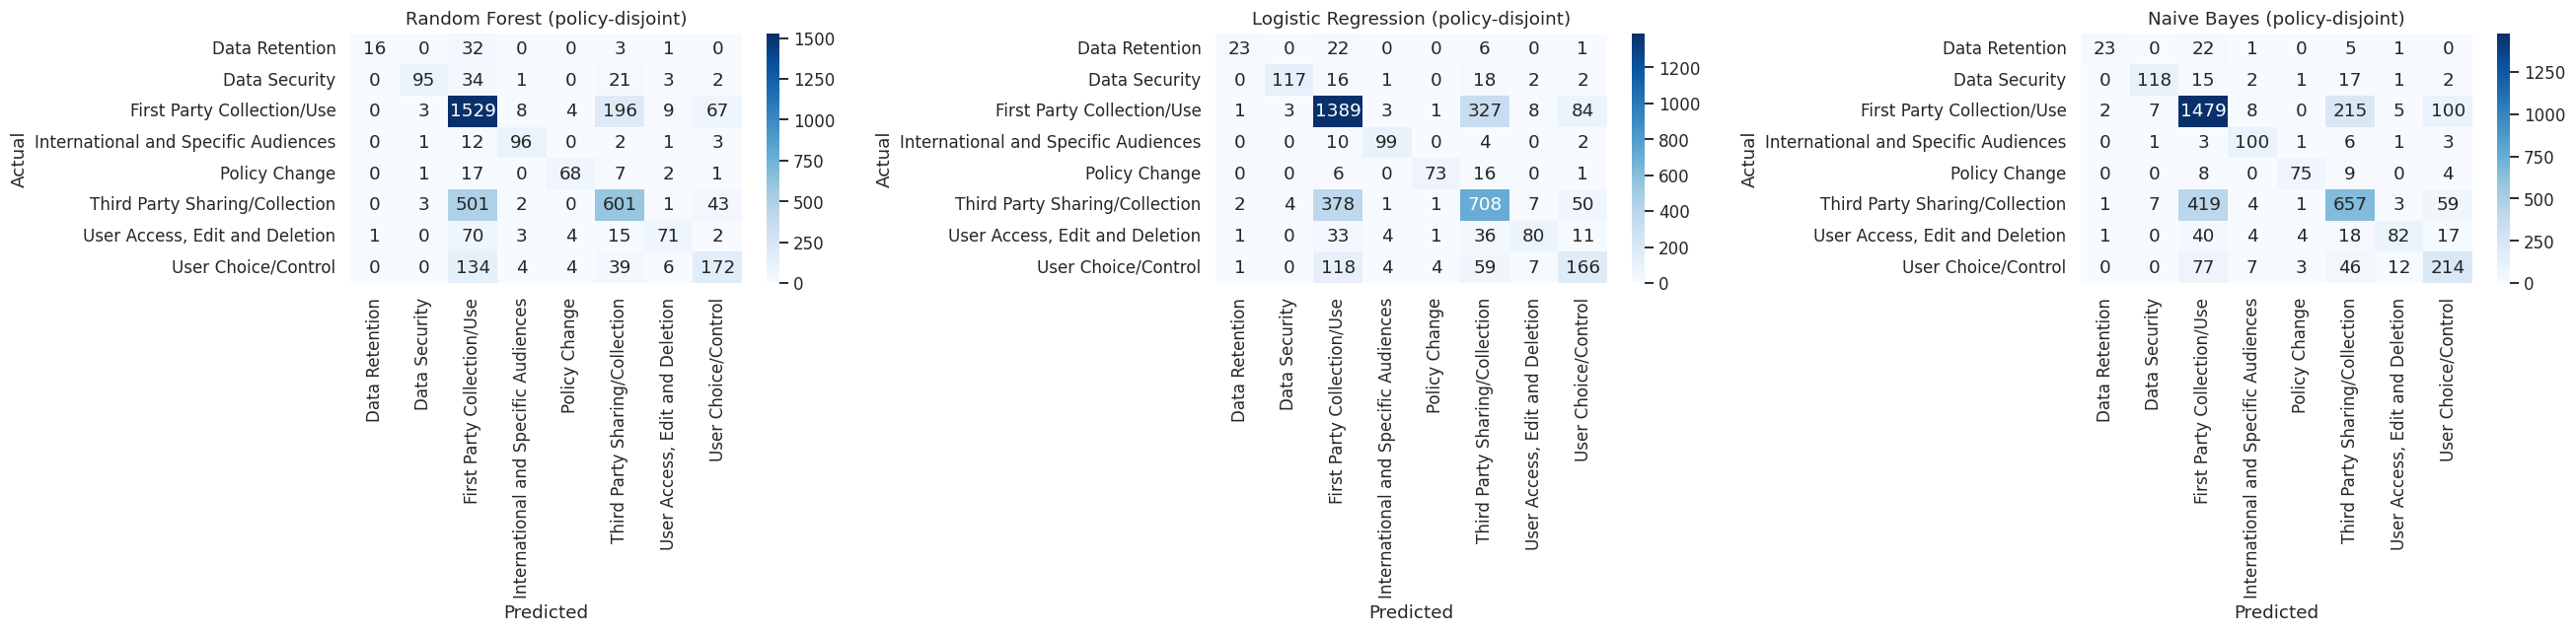
\includegraphics[width=\textwidth]{figures/confusion_matrices_classical.png}
\caption{Confusion matrices (raw counts) for the three classical models on the policy-disjoint test set.}
\label{fig:confusion}
\end{figure*}

\subsection{Best and Worst Configurations}

Among the 60 tuning runs, the winning configuration for BERT Base under the policy-disjoint scheme is learning rate $3 \times 10^{-5}$, batch size 32 (validation macro-F1 0.723, test macro-F1 0.706). The winning classical configuration is Naive Bayes with $\alpha = 0.05$ (validation macro-F1 0.680, test macro-F1 0.701). The weakest configuration across all models is SimpleRNN with embed=128, hidden=64, dropout=0.3, $lr=10^{-3}$ under the policy scheme (validation macro-F1 0.110).

\subsection{Representation Status}

TF-IDF is the only representation with completed downstream classification; every classical model result in Table~\ref{tab:results} uses TF-IDF. The Word2Vec pipeline was implemented but not executed for completed downstream classification. GloVe was not implemented. BERT Base results come from partial, layer-frozen fine-tuning; no full fine-tune was attempted.

\section{Cross-Jurisdictional External Validation on Bangladeshi Privacy Policies}
\label{sec:bd}

Sections~\ref{sec:methodology}--\ref{sec:conclusion} evaluate models entirely within OPP-115: every train, validation, and test row comes from the same 115-policy, US-centric corpus. This section reports a new study, external to OPP-115 in the strictest sense --- applying the policy-disjoint BERT Base model (Table~\ref{tab:results}, macro-F1 0.706\footnote{The value obtained when independently re-running this checkpointing and inference pipeline was 0.6914; both figures come from the same configuration and are within expected run-to-run fine-tuning variance. Table~\ref{tab:results}'s 0.706 is retained throughout this section for internal consistency with Iteration 1.}) to real privacy policies published by companies with no representation whatsoever in the training data.

\subsection{Motivation}

OPP-115 is a US-centric snapshot: all 115 source policies are American company policies, collected under a US regulatory backdrop. Bangladesh has no direct equivalent of GDPR or CCPA in force, and a fast-growing set of digital-first companies (mobile financial services, e-commerce, fintech) whose privacy policies are a comparatively recent artifact rather than a mature legal genre. If a classifier trained purely on OPP-115 produces a plausible, appropriately-uncertain category distribution on Bangladeshi text, that is evidence it has learned category-level structure that generalizes past OPP-115's specific vocabulary and drafting conventions --- not just memorized US boilerplate, a question directly motivated by the same leakage-and-memorization concern (Section~\ref{sec:methodology}) that motivates this paper's split-scheme comparison in the first place.

This is explicitly a \textbf{Tier 1 (Primary study), descriptive} study: no manually-annotated ground truth exists for the Bangladeshi text used here. A Tier 2 study --- manual annotation of a Bangladeshi sample against the same eight-category schema, to obtain real precision/recall/macro-F1 --- is scoped as future work (Section~\ref{sec:future}) and not attempted in this iteration.

\subsection{Closing the Checkpointing Gap}

The executed project notebook trains BERT Base for both split schemes entirely in memory: the fitted model is scored and discarded when the kernel session ends, and only the TF-IDF vectorizer and cached embedding arrays are ever written to disk. Before any transfer experiment was possible, this iteration added the missing step --- \texttt{model.save\_pretrained()} and \texttt{tokenizer.save\_pretrained()} immediately after the policy-disjoint scheme's winning configuration, plus a label-index mapping recorded at training time. This step was first validated as an independently-runnable script that reproduced Table~\ref{tab:results}'s BERT Base policy-disjoint result to within run-to-run fine-tuning variance (Section~\ref{sec:bd}, footnote above), then added directly to the training notebook so the checkpoint is produced automatically by any future run.

\subsection{Bangladeshi Company Subset}

A source index of 100 Bangladeshi companies and their privacy-policy URLs was narrowed to 35 by taking the ten largest represented sectors in full, rather than a uniform sample across all represented sectors, so each sector retains enough companies for a sector-level view rather than 35 singletons: Banking (8), Telecommunications (4), Mobile Financial Services (3), E-commerce (3), E-commerce Marketplace (3), Retail and Consumer Goods (3), Healthcare and Diagnostics (3), Healthcare Provider (3), News Media (3), and Software and IT (2).

A plain HTTP GET plus HTML text extraction (no headless browser) successfully retrieved usable text for 26 of these 35 companies. Three failed outright with connection or SSL errors; six more returned a technically successful response under 500 characters of extracted text --- JavaScript-rendered single-page applications whose real content is never present in the server-rendered HTML a plain GET receives. This 74\% usable rate is itself a data point about the Bangladeshi corporate web ecosystem, and the 26\% attrition is a selection effect worth naming: companies reachable by a static scraper may differ systematically (technical sophistication, site simplicity) from those excluded.

\subsection{Inference Pipeline}

For each of the 26 usable companies: (1) page text is split into candidate sentences with an NLTK sentence tokenizer, filtered to 4--120 words to discard navigation fragments, rather than segmented at clause level --- directly following Section~\ref{sec:methodology}'s multi-practice-clause finding (34.9\% of OPP-115 clauses carry more than one category), which motivates avoiding clause-level input for a model trained on single-category spans; (2) each sentence is cleaned with the identical \texttt{minimal} preprocessing variant used at BERT training time (Table~\ref{tab:preprocess}), so inference-time text matches train-time text distributionally; (3) the checkpointed model classifies each sentence in batches, recording the arg-max category and its softmax probability as a confidence score.

\subsection{Results}

3,120 sentences were classified across the 26 companies; overall mean prediction confidence was 0.713. Table~\ref{tab:bdresults} compares the resulting predicted category distribution against OPP-115's ground-truth distribution; Figure~\ref{fig:bd_comparison} visualizes the same comparison.

\begin{table}[t]
\centering
\footnotesize
\setlength{\tabcolsep}{3pt}
\begin{tabularx}{\columnwidth}{@{}Xccc@{}}
\toprule
\textbf{Category} & \textbf{OPP-115} & \textbf{BD (pred.)} & \textbf{Conf.} \\
\midrule
Third Party Sharing/Collection & 27.76\% & 21.70\% & 0.725 \\
User Choice/Control & 9.66\% & 4.87\% & \textbf{0.550} \\
User Access, Edit \& Deletion & 3.97\% & 2.60\% & 0.673 \\
Int'l and Specific Audiences & 3.05\% & 2.63\% & 0.640 \\
Policy Change & 2.63\% & 4.39\% & 0.810 \\
First Party Collection/Use & 46.97\% & 48.78\% & 0.723 \\
Data Retention & 1.93\% & 4.10\% & 0.612 \\
Data Security & 4.03\% & 10.93\% & \textbf{0.740} \\
\bottomrule
\end{tabularx}
\caption{OPP-115 ground-truth category share vs. BD predicted category share (3,120 sentences, 26 companies), with BD mean prediction confidence per category.}
\label{tab:bdresults}
\end{table}

\begin{figure}[t]
\centering
\includegraphics[width=0.95\columnwidth]{figures/bd_category_comparison.png}
\caption{Category distribution: OPP-115 ground truth vs. BD predicted, BERT Base policy-disjoint checkpoint.}
\label{fig:bd_comparison}
\end{figure}

The overall shape is preserved: First Party Collection/Use is the plurality category in both corpora (46.97\% vs. 48.78\%), and the rank order of the top three categories matches. Two divergences dominate, in opposite directions: Data Security is over-predicted by 6.90 percentage points at above-average confidence (0.740), and User Choice/Control is under-predicted by 4.79 points at the lowest confidence of any category (0.550).

\subsection{Discussion}

The two largest gaps carry different evidentiary weight given their confidence. \textbf{Data Security's} higher-than-average confidence makes it the more credible of the two as a real effect --- plausibly sectoral rather than (or in addition to) jurisdictional, since 11 of the 26 usable companies are banks, mobile-financial-service providers, or fintech-adjacent, sectors where security language is a standard disclosure even in otherwise short policies. \textbf{User Choice/Control's} combination of the largest confidence deficit and this being the model's own second-weakest OPP-115 category by F1 (Table~\ref{tab:perclass}, 0.59) is the clearer domain-shift signal: the model is already comparatively unreliable on this category in-distribution, and its confidence drops further out-of-distribution, consistent with BD-specific choice/consent language (e.g., NID-verification flows, BTRC-regulated consent mechanisms) differing enough from OPP-115's US-centric phrasing that the fine-tuned tokenizer's training data never modeled it well.

This distinction --- a same-direction, high-confidence gap read as more likely genuine, versus a gap coinciding with a category the model already struggles with, read as more likely domain shift --- is the paper's proposed practical takeaway for applying any trained classifier outside its training distribution without new labels: per-category confidence is not just a byproduct of the softmax, but a usable, label-free diagnostic.

Sectoral composition is a confound this tier cannot separate from a jurisdictional effect: OPP-115's own sector mix is not reproduced in the 26-company BD subset, and a sector-matched comparison (Section~\ref{sec:future}) is required before attributing the Data Security gap to jurisdiction rather than industry norms.

\section{Discussion and Findings}

Our central finding is that a conventional stratified split, scored on accuracy or on an unexamined single-split macro-F1, would have led to incorrect conclusions about model ranking. Several recurrent architectures would be ranked well above their honest positions, silently, with nothing in the leaky split's own numbers to flag the problem.

The document-level structure in privacy policies is extreme but not unique: contracts, regulatory filings, terms of service, and form letters all exhibit similar template reuse. Our findings suggest that any text classification task built on such documents should adopt document-grouped evaluation as standard practice.

The cross-jurisdictional result (Section~\ref{sec:bd}) extends this paper's leakage-and-generalization theme one step further: a model selected specifically for honest, policy-disjoint generalization is also the model best positioned to be usefully applied outside its training distribution altogether, and the same discipline that motivated evaluating it honestly --- distrusting an apparently good score until its source is examined --- motivates treating a plausible-looking predicted distribution on new, unlabeled data as informative but not conclusive without confidence diagnostics or, eventually, real labels.

\section{Conclusion}
\label{sec:conclusion}

We systematically compare evaluation protocols for privacy-practice classification across three classical, six recurrent, and one transformer model, and, in this iteration, transfer the resulting best model to an out-of-distribution jurisdiction. Our key findings are:

\begin{enumerate}
\item Evaluating on a conventional row-level split changes not just the absolute numbers but which model appears to win (RQ1).
\item The evaluation-protocol gap is largest for recurrent architectures trained from scratch and smallest for BERT Base and classical models (RQ2).
\item Under honest, policy-disjoint evaluation, BERT Base leads at macro-F1 0.706, narrowly ahead of Naive Bayes (0.701); the classical models' competitiveness suggests that privacy-practice categories carry strong lexical cues that TF-IDF captures effectively on short spans (RQ3).
\item \textbf{2nd Phase(Application in Bangladeshi Company Policy's dataset)} Applied without retraining to 3,120 sentences from 26 Bangladeshi companies, the same policy-disjoint BERT Base model produces a predicted category distribution that largely preserves OPP-115's shape, with per-category confidence distinguishing a likely-real sectoral gap (Data Security, +6.9pp, confidence 0.740) from a likely domain-shift artifact (User Choice/Control, $-$4.8pp, confidence 0.550, also this model's weakest OPP-115 category) (RQ4).
\end{enumerate}

We take the leakage-versus-honest contrast, and the cross-jurisdictional transfer result it enabled, as evidence that document-grouped evaluation and confidence-aware, label-free diagnostics should both be standard practice when a text classifier is applied beyond the corpus it was validated on.

\section{Limitations}

The six recurrent models process every padded position in a 48-token sequence without length masking; short spans continue being processed through trailing padding, which may partly explain the recurrent family's large evaluation-protocol gap. The executed pipeline applied base preprocessing to the recurrent models rather than the designed lemmatized variant; the isolated effect is untested. Random seeds are not reset per configuration inside the recurrent tuning loop. Only TF-IDF downstream classification is complete; Word2Vec was not evaluated and GloVe was not implemented. BERT results come from partial, layer-frozen fine-tuning rather than a full fine-tune. All results are oracle-span: a deployed system would additionally need an upstream span-detection step.

The Bangladeshi external-validation study (Section~\ref{sec:bd}) carries additional, tier-specific limitations: it is descriptive only, with no manually-labeled BD ground truth against which to compute real precision or recall; it covers 26 companies concentrated in ten sectors at a single collection snapshot, not a representative sample of the Bangladeshi corporate sector; 26\% of the sampled companies were unreachable by a static scraper, a selection effect on which companies are represented; sentence-level segmentation approximates but does not reproduce OPP-115's annotator-drawn spans; and no statistical significance testing (e.g., chi-square per category) is applied to the reported percentage-point gaps.

\section{Future Work}
\label{sec:future}

The most pressing fixes are:
\begin{enumerate}
\item Retrain the six recurrent models with length-aware packing and per-configuration seed resets.
\item Complete the Word2Vec downstream evaluation.
\item Apply the designed lemmatized preprocessing to recurrent models to isolate its effect.
\item Feed span-plus-clause context to specifically help the First Party versus Third Party confusion.
\item Implement minority-class-aware training strategies for Data Retention.
\item Execute a full, non-frozen BERT fine-tune given a larger compute/time budget.
\item \textbf{2nd Phase(Application in Bangladeshi Company Policy's dataset)} Conduct the Tier 2 validation: manually annotate 200--300 Bangladeshi sentences (ideally with two annotators, mirroring OPP-115's own multi-annotator design) against the same eight-category schema to obtain real precision/recall/macro-F1 on Bangladeshi text.
\item \textbf{2nd Phase(Application in Bangladeshi Company Policy's dataset)} Add a headless-browser fallback (e.g., Playwright) for the six JavaScript-rendered companies excluded in this iteration, and a retry strategy for the three outright failures, before scaling the subset past 35 companies.
\item \textbf{2nd Phase(Application in Bangladeshi Company Policy's dataset)} Construct a sector-matched pairing against OPP-115 companies, with chi-square and paired-comparison testing on a disclosure index, to separate the sectoral confound identified in Section~\ref{sec:bd} from a genuine jurisdictional effect.
\end{enumerate}

\section*{Acknowledgments}

This work was conducted as part of the CSE440 course project at BRAC University. We thank the annotators of the OPP-115 corpus and the maintainers of the datasets and libraries used in this research.

\bibliography{custom}
\bibliographystyle{plainnat}

\end{document}
